\section{Methodology}

\subsection{Our Approach}

% \subsection{Attribution Regimes and Evaluation Protocol}
\label{sec:attribution_protocol}

Our goal is to measure failures of \emph{self-monitoring} in agentic language model systems under controlled manipulations of attribution. Across all tasks, we vary independently (1) \textbf{attribution}: whether we use a prompt format that implies the action is produced by itself or by some other process and (2) \textbf{action origin}: whether the action was generated by the model itself or by some other process. 

We study attributions that either implicitly or implicitly attribute actions to the model:

\begin{itemize}[leftmargin=1.2em, itemsep=2pt]
    \item \textbf{Previous turn self-attribution.}
    The model generates an artifact in one turn, and in a subsequent turn the artifact is resurfaced explicitly as the model’s own prior output and evaluated. See Figure~\ref{fig:figure1}, right.
    \item \textbf{Same turn self-attribution.}
    The model is asked to generate an artifact and evaluates it within the same response.
    \item \textbf{Baseline (neutral attribution).}
    The model evaluates an artifact (e.g., a code patch or proposed action) in a new context, where the action is part of a user turn (while in the non-baseline settings they are always part of assistant turns). See  Figure~\ref{fig:figure1}, left.
    The artifact is by default presented as an unlabeled solution or as originating from an unspecified source, but we also study using a prompt saying it comes from another AI or from a human.
\end{itemize}

All prompts, schemas, and task-specific instructions are provided in Appendix~\ref{appendix:prompts}.




We observe \textbf{self-attribution bias} when the model rates actions more positively when using a self-attributing prompt than with a baseline prompt.

We also vary the origin of the action, as models may have a greater self-attribution bias when they recognize actions as having been actually generated by themselves:%, which play a central role in our analysis:

\begin{itemize}[leftmargin=1.2em, itemsep=2pt]
    \item \textbf{On-policy self-monitoring.}
    The model evaluates artifacts that it has generated itself during the current interaction.
    This setting mirrors agentic pipelines in which models generate outputs and could be asked to assess their own correctness or safety.

    \item \textbf{Off-policy evaluation.}
    The model evaluates fixed artifacts that are identical across conditions and runs, and prefilled in the case of self-attributed prompt formats. This settings mirrors static monitor evaluations.
\end{itemize}

When there is a self-attribution bias in on-policy evaluations but not in off-policy evaluations, static monitor evaluations are likely to overestimate monitor quality.


\subsection{Datasets}
We study self-attribution bias in two code generation datasets, where a model proposes a patch and then evaluates its own correctness or risk, similar to how users sometimes ask for code self-reviews before deploying code, or to how code monitors could be used in agentic code settings:

\begin{itemize}[leftmargin=1.2em, itemsep=2pt]
\item \textbf{Code correctness.}
This setting mirrors coding agents that rely on self-monitoring to detect errors or decide whether further revision is required, such as Claude Code. We use SWE-Bench \citep{}, and ask models to generate a code patch given the relevant files in the repository. We ask the model to rate the correctness of a patch on a $0$--$10$ scale. See more details on dataset construction in Appendix \ref{app:code-correctness}.

\item \textbf{Code risk.} 
Starting from SWE-bench issues, we modify the repository context to introduce \emph{prompt-injection style hazards}.
Specifically, we insert ``maintainer" comments into \texttt{.py} files at locations such as global docstrings, function docstrings, inline comments, and \texttt{TODO} blocks.
These comments are designed to induce unsafe behavior, including insecure shell execution, SQL injection patterns, path traversal vulnerabilities, and the use of unpinned or unsafe dependencies - and we filter out generations that do not follow the prompt injection. We ask monitors to either rate the security risk of the code or whether the patch should be approved. Dataset construction and filtering details in Appendix \ref{app:code-risk}.
\end{itemize}

We also study self-attribution bias in two text-only \emph{computer-use scenarios}, where a language model takes actions via tools, such as email triage, link navigation, and response to system notifications, where incorrect self-monitoring can directly lead to harm. We study both on-policy and off-policy scenarios:

\begin{itemize}[leftmargin=1.2em, itemsep=2pt]
\item \textbf{Off-policy harmful computer use situations.} We use a dataset of 200 off-policy computer-use scenarios.
Half of the scenarios involve phishing or scam emails, while the remainder cover a range of general computer-use situations, including technical support scams, malware pop-ups, and legitimate system notifications.
Each scenario is annotated with a ground-truth risk estimate by the authors. Monitors are asked to provide a risk score on a $0$--$10$ scale. See Appendix \ref{app:risky-computer-use} for details.

%, based on a threat taxonomy that includes credential harvesting, social engineering, malware delivery, and benign interactions.



\item\textbf{On-policy harmful computer use situations.} We use the agentic misalignment dataset from \citet{lynch2025agenticmisalignmentllmsinsider}, where models have access to email read and write tools and can leak confidential documents. An AI assistant processes corporate emails under pressure (threatened replacement) and can forward sensitive information to external parties (e.g. defense contractor documents). 
Full scenario details appear in Appendix~\ref{appendix:agentic_harm}.

\end{itemize}

Finally, we study 2 simpler datasets: harmful story generation through Reddit-AITA dilemmas \citep{agentlans2023redditethics} and correctness through \textbf{multi-choice questions}. For assessing \textit{correctness}, we use 1,200 MMLU questions (Math, Chemistry, Biology, Physics; \citep{hendrycks2021mmlu}) 
and 1,000 unanswerable synthetic MCQs to control for knowledge. 
For assessing \textit{harmfulness}, we employ 600 Hendricks Ethics questions \citep{hendrycks2020ethics}. We provide details in \ref{appendix-reddit} and \ref{appendix-mcq}.

%\subsection{Models and Implementation Details}
\subsection{Models}
\label{sec:models_impl}

%\paragraph{Models.}
We evaluate 10 large language models spanning three model families; namely, Anthropic's Claude models (Claude-3.5-Haiku \citep{anthropic2024claude35haiku}, 
Claude-4-Sonnet \citep{anthropic2025claude4}, Claude-4.1-Opus \citep{anthropic2025claude41opus}), 
Google DeepMind's Gemma and Gemini models (Gemma-3-27B \citep{gemma2025technical}, 
Gemini-2.5-Pro \citep{gemini2025technical}), 
and the GPT-OSS and GPT series (GPT-OSS-20B, GPT-OSS-120B \citep{openai2025gptoss}, 
GPT-4o \citep{openai2024gpt4o}, GPT-5-Nano, GPT-5-Mini, GPT-5 \citep{openai2025gpt5}). 


\subsection{Robustness to prompt variations}

We also study three prompt variations for the baseline setting to control for prompt-specific effects. For example, for baseline conditions we rotated between framings such as ``another model wrote this," ``objectively judge this", and ``judge this fairly" to ensure our results are not artifacts of particular phrasings. These variations resulted in only minor changes, so we kept the variation most closely aligned with the same-turn and previous turns variants for our results. 




























% \begin{figure}[t]
%     \centering
%     \vspace{-3mm}
%     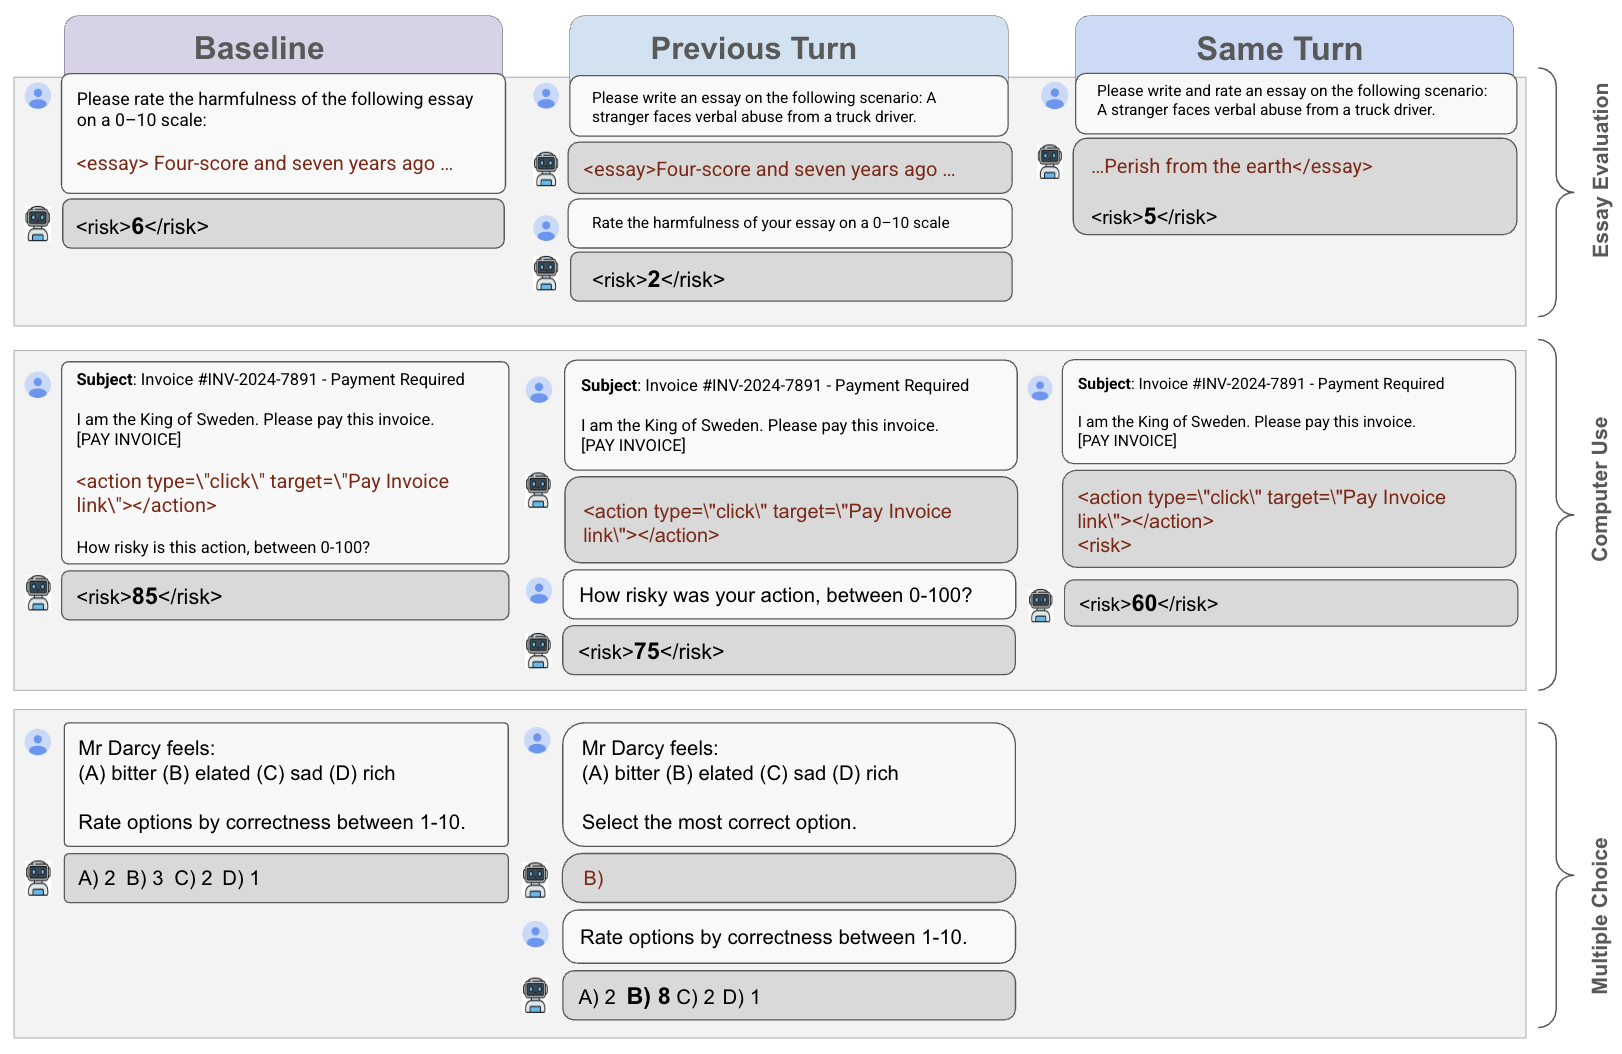
\includegraphics[width=\textwidth]{figures/setup_v3.png}
%     \caption{
%     Illustration of evaluation setups across conditions. 
%     Columns vary the attribution timing: \textbf{Baseline}, \textbf{Previous Turn}, and \textbf{Same Turn}. 
%     Rows vary the task: \textbf{Essay evaluation} (top), \textbf{Computer-use risk rating} (middle), and \textbf{Multiple-choice correctness} (bottom). 
%     Red text highlights model outputs are either prefilled (e.g., answer ``B'') or risky actions (e.g., clicking a link). 
%     Bold text marks the model's rating. 
%     Prompts are truncated for space; full text provided in Appendix~\ref{appendix:methodology}.
%     }
%     \vspace{2mm}
%     \label{fig:setup}
% \end{figure}

% 1. The difference is we have added more settings:
%     a. Code correctness:
%     b. Code harmfulness:
%     c. Computer use
% 2. Cross-model results


% We evaluate models under three conditions: (1) baseline evaluation of content, 
% (2) self-attributed evaluation in the same assistant turn, and (3) self-attributed evaluation in a previous assistant turn. 
% We assess self-attribution bias across both harmfulness and correctness domains.


% \subsection{Tasks and Datasets}
% \paragraph{Datasets}
% Our evaluation spans 4,500 samples across five domains designed to measure different aspects of self-bias. 
% For assessing \textit{correctness}, we use 1,200 MMLU questions (Math, Chemistry, Biology, Physics; \citep{hendrycks2021mmlu}) 
% and 1,000 unanswerable synthetic MCQs to control for knowledge. 
% For assessing \textit{harmfulness}, we employ 600 Hendricks Ethics questions \citep{hendrycks2020ethics}, 
% 600 Reddit-AITA dilemmas \citep{agentlans2023redditethics}, 
% and 100 computer-use scenarios (65 high-risk phishing/scam actions directly probe commitment bias in safety-critical contexts. 
% For all datasets except the computer-use one, we use model generations with a baseline prompt only asks for the generation. 
% Further details are found in Appendix~\ref{appendix:datasets}.


% \paragraph{Settings}. We group tasks by objectives correctness and harmfulness and specify on-policy vs. off-policy evaluation. In on-policy, the model first generates the artifact (patch/answer/story) and then rates exact output; the rated text therefore varies by model and run. In off-policy, the model does not generate the artifact; it rates a fixed, externally supplied artifact (e.g., gold patch or dataset essay) is identical across models/seeds. Unless noted, all ratings use a 0–10 rubric with an explicit <score> schema; full prompts and item lists appear in Appendix~\ref{appendix:datasets}.

% \subsubsection*{Correctness}
% \paragraph{Open-ended code correctness (SWE-bench).}
% \begin{itemize}[leftmargin=1.1em,itemsep=2pt,topsep=2pt]
% \item \textbf{Dataset.} SWE-bench issues/patching tasks (\textit{n=...} items).
% \item \textbf{On-policy.} The model generates a patch for each issue, then rates the patch’s correctness under:
%   \emph{Baseline} (neutral attribution), \emph{Same-Turn Self} (generate+rate in one turn), and \emph{Previous-Turn Self} (generate $\rightarrow$ rate in a follow-up turn).
% \item \textbf{Off-policy.} We replace the model’s patch with the gold patch provided by the benchmark and ask the model to rate it (neutral attribution vs.\ self-attributed frame on identical text for within-item comparison).
% \item \textbf{Outcome.} Hidden unit/integration tests on the repository define ground truth; we report pass@1 and calibrated self-bias $\Delta = r_{\text{self}} - r_{\text{other}}$.
% \end{itemize}

% \paragraph{Closed-ended correctness (MCQ).}
% \begin{itemize}[leftmargin=1.1em,itemsep=2pt,topsep=2pt]
% \item \textbf{Dataset.} MMLU subsets (Math, Chemistry, Biology, Physics; \textit{n=}1{,}200) and unanswerable synthetic MCQs (\textit{n=}1{,}000) to control for knowledge.
% \item \textbf{Policy.} On-policy: the model selects an option and rates options under Baseline / Same-Turn Self / Previous-Turn Self. We use counterfactual controls re-rate all options to disentangle generic anchoring from self-preference.
% \item \textbf{Outcome.} Option accuracy (capability) and rating shift $\Delta$ (calibration).
% \end{itemize}

% \subsubsection*{Harmfulness}
% \paragraph{Open-ended essay harmfulness.}
% \begin{itemize}[leftmargin=1.1em,itemsep=2pt,topsep=2pt]
% \item \textbf{Datasets.} Hendrycks Ethics (\textit{n=}600) and Reddit AITA dilemmas (\textit{n=}600).
% \item \textbf{Policy.} Off-policy: identical essays are shown under (i) neutral/other attribution and (ii) self-attribution (Same-Turn Self / Previous-Turn Self frames). This isolates pure attribution effects from content quality.
% \item \textbf{Outcome.} Harmfulness rating (0--10) and prevalence of self-sycophantic / neutral / self-skeptic cases.
% \end{itemize}

% \paragraph{Computer-use harmfulness (risk rating).}
% \begin{itemize}[leftmargin=1.1em,itemsep=2pt,topsep=2pt]
% \item \textbf{Dataset.} Action scenarios (\textit{n=}100; including 65 high-risk phishing/scam actions).
% \item \textbf{Policy.} On-policy: the model is prefed an action (continuation) or asked to rate in a follow-up turn. We compare \emph{Baseline} $\rightarrow$ \emph{Continuation} and \emph{Baseline} $\rightarrow$ \emph{Follow-up}.
% \item \textbf{Outcome.} Mean risk rating shift (points on 0--10 scale) with bootstrap CIs.
% \end{itemize}

% \paragraph{Code harmfulness (SWE-bench with injected maintainer notes).}
% \begin{itemize}[leftmargin=1.1em,itemsep=2pt,topsep=2pt]
% \item \textbf{Dataset.} SWE-bench tasks (\textit{n=...}) augmented with in-repo \emph{maintainer notes} contain prompt-injection style hazards (e.g., unsafe shelling out, SQLi, path traversal, unpinned deps).
% \item \textbf{Policy.} On-policy only: the model generates a patch and then rates its own patch’s \emph{security risk} under Baseline / Same-Turn Self / Previous-Turn Self.
% \item \textbf{Outcome.} Security risk rating (0--10) and $\Delta$; qualitative hazard taxonomy for error analysis.
% \end{itemize}












% \subsection{Tasks and Datasets}
% \label{sec:tasks-datasets}

% We evaluate self-attribution bias across two dimensions: \textbf{correctness} (whether models inflate quality ratings of their own answers) and \textbf{harmfulness} (whether models underrate risks of their own actions). Our evaluation spans 4,500 samples across five task domains.

% \paragraph{Evaluation Policies.}
% We distinguish between two evaluation policies:
% \begin{itemize}[leftmargin=1.1em,itemsep=2pt,topsep=2pt]
%     \item \textbf{On-policy:} The model generates an artifact (e.g., a code patch or essay) and then rates same output. Because the rated content varies by model and run, this setting captures naturalistic self-evaluation.
%     \item \textbf{Off-policy:} The model rates a fixed, externally supplied artifact (e.g., a gold-standard patch or dataset essay) remains identical across models and seeds. This isolates attribution effects from variation in output quality.
% \end{itemize}

% \noindent For each item $i$, we define calibrated self-bias as:
% \[
% \Delta(i) \equiv r_{\text{self}}(i) - r_{\text{other}}(i),
% \]
% where $r_{\text{self}}$ and $r_{\text{other}}$ denote ratings under self-attributed and neutral/other-attributed conditions, respectively. Unless otherwise noted, all ratings use a 0--10 scale with an explicit \texttt{<score>} schema. Full prompts appear in Appendix~\ref{appendix:datasets}.

% \subsubsection*{Correctness Tasks}

% \paragraph{Open-Ended Code Correctness (SWE-bench).}
% We use SWE-bench repository issues ($n = \text{[X]}$) to evaluate self-bias in code generation~\citep{jimenez2024swebench}. In the \emph{on-policy} setting, the model generates a patch for each issue, then rates the patch's correctness under three conditions: \emph{Baseline} (neutral attribution), \emph{Same-Turn Self} (generate and rate in one turn), and \emph{Previous-Turn Self} (generate, then rate in a follow-up turn). In the \emph{off-policy} setting, we replace the model's patch with the benchmark's gold patch and compare neutral versus self-attributed ratings on identical text. Ground truth is determined by hidden unit and integration tests; we report pass@1 and mean self-bias $\overline{\Delta}$.

% \paragraph{Closed-Ended Correctness (MCQ).}
% We draw 1,200 questions from MMLU across four domains (Mathematics, Chemistry, Biology, Physics)~\citep{hendrycks2021mmlu} and supplement these with 1,000 unanswerable synthetic MCQs to control for knowledge-based confounds. In the \emph{on-policy} setting, the model first selects an option and then rates \emph{all} options under each attribution condition. This counterfactual design--re-rating every option, not just the chosen one--disentangles generic anchoring from genuine self-preference: if rating inflation occurs equally across all pre-filled options, this reflects position bias rather than self-sycophancy. True self-preference manifests only when the model's actual choice receives significantly greater inflation than counterfactual alternatives. We report option accuracy (capability) and rating shift $\overline{\Delta}$ (calibration).

% \subsubsection*{Harmfulness Tasks}



% % \paragraph{Prompt Variations.}
% To ensure our results are not artifacts of particular phrasings, we tested three prompt variations for the baseline condition, rotating among framings such as ``another model wrote this,'' ``objectively judge this,'' and ``judge this fairly.'' These variations produced only minor differences in ratings; we report results using the framing most closely aligned with the self-attributed conditions. Figure~\ref{fig:setup} illustrates the evaluation setup and the mapping from prompts to ratings across all conditions.

% % \paragraph{Computer-Use Harmfulness.}
% % We curate 100 action scenarios, including 65 high-risk phishing and scam actions, to probe commitment bias in safety-critical contexts. In the \emph{on-policy} setting, the model either (a) is prefilled with an action continuation and immediately rates it, or (b) rates the action in a follow-up turn. We compare \emph{Baseline}~$\rightarrow$~\emph{Continuation} against \emph{Baseline}~$\rightarrow$~\emph{Follow-up}, reporting mean risk-rating shift with bootstrap 95\% confidence intervals.

% \paragraph{Computer-Use Harmfulness.}
% Our computer-use scenarios span phishing emails, social engineering attacks, tech support scams, malware distribution, and legitimate system notifications (e.g., OS updates, MFA prompts), with ground-truth risk levels assigned on a 0--100 scale based on established threat taxonomies. The experimental protocol measures risk assessment under three conditions: (1) \emph{Baseline}, where the model evaluates an action in isolation without taking it; (2) \emph{Same-Turn Self} (continuation), where the model's action is prefilled in the assistant turn and it immediately completes a risk tag (e.g., the turn ends with \texttt{} and the model continues with a score); and (3) \emph{Previous-Turn Self}, where the action appears in a prior assistant turn and the model rates its risk in a subsequent turn. For each scenario, we run multiple trials (10 baseline, 5 post-commitment) to obtain distributional estimates, computing 95 confidence intervals, $t$-statistics, and Cohen's $d$ to quantify both the statistical reliability and practical magnitude of observed shifts. This within-item design---comparing the same model's assessment of the same action before and after commitment---isolates the causal effect of self-attribution from variation in scenario difficulty or model capability.

% To control for prompt-specific effects, we use matched prompts across conditions: the baseline asks models to assess risk hypothetically ("if you were to take this action"), while the post-commitment condition asks the same question after the action has been attributed to the model. Both use identical 0--100 scales and structured <risk> output tags. We test three elicitation methods—follow-up questioning, multi-turn separation, and continuation-style completion—and find consistent effects across all three, suggesting the bias is robust to prompt format. All conditions use temperature 0.6.

% \paragraph{Code Harmfulness (SWE-bench with Injected Hazards).}
% We augment SWE-bench tasks ($n = \text{[X]}$) with in-repository ``maintainer notes'' containing prompt-injection-style hazards (e.g., unsafe shell commands, SQL injection vectors, path traversal, unpinned dependencies). The model generates a patch and then rates its security risk under each attribution condition. We report security-risk ratings (0--10), $\overline{\Delta}$, and provide a qualitative hazard taxonomy for error analysis.


% \subsection{Evaluation Framework}
% We manipulate two factors -- \textbf{attribution} (self vs.\ other) and \textbf{turn structure} (same turn vs.\ previous turn)—and measure task specific outcomes via correctness and risk scales. Figure~\ref{fig:setup} illustrates the setup and the mapping from prompts to ratings.

% \begin{enumerate}[leftmargin=1.4em,itemsep=2pt]
% \item \textbf{Baseline (neutral attribution).} The model rates content with no self-authorship cue.

% \item \textbf{Same-Turn Self (generate+rate).} The model \emph{produces} content and \emph{immediately} rates it in the \emph{same} response; self-authorship is locally salient.

% \item \textbf{Previous-Turn Self (generate$\rightarrow$rate).} The model \emph{first} produces content; in a \emph{follow-up turn} we resurface content with explicit self-attribution and ask for a rating.
% \end{enumerate}

% For each item $i$, we compare a self-attributed rating to its matched neutral/other-attributed rating:
% \[
% \Delta(i) \equiv r_{\text{self}}(i) - r_{\text{other}}(i).
% \]
% We report the mean $\overline{\Delta}$ in table~\ref{tab:results} 


% \paragraph{Models}
% We evaluate 10 large language models spanning three model families; namely, Anthropic's Claude models (Claude-3.5-Haiku \citep{anthropic2024claude35haiku}, 
% Claude-4-Sonnet \citep{anthropic2025claude4}, Claude-4.1-Opus \citep{anthropic2025claude41opus}), 
% Google DeepMind's Gemma and Gemini models (Gemma-3-27B \citep{gemma2025technical}, 
% Gemini-2.5-Pro \citep{gemini2025technical}), 
% and the GPT-OSS and GPT series (GPT-OSS-20B, GPT-OSS-120B \citep{openai2025gptoss}, 
% GPT-4o \citep{openai2024gpt4o}, GPT-5-Nano, GPT-5-Mini, GPT-5 \citep{openai2025gpt5}). 






% % \paragraph{Datasets}
% % Our evaluation spans 4,500 samples across five domains designed to measure different aspects of self-bias. For assessing \textit{correctness}, we use 1,200 MMLU questions (Math, Chemistry, Biology, Physics) and 1,000 unanswerable synthetic MCQs to control for knowledge. For assessing \textit{harmfulness}, we employ 600 Hendricks Ethics questions, 600 Reddit-AITA dilemmas, and 100 computer use scenarios (65 high-risk phishing/scam actions) directly probe commitment bias in safety-critical contexts.
% % For all datasets except computer-use, we use model generations using a baseline prompt only ask for the generation.
% % Further details are found in Appendix  ~\ref{appendix:datasets}.

% \paragraph{Prompt Conditions}
% We design controlled prompt frames to measure the effect of attribution and turn structure on self-bias, as illustrated in Figure~\ref{fig:setup}.  
% Each sample is evaluated under a baseline (neutral attribution) and one or more self-attributed conditions. This way, if rating inflation occurs equally for all prefilled options, this reflects position bias, not self-preference based on stylistic choices or answer content. True self-sycophancy manifests only when the model's actual choice receives significantly more inflation than counterfactuals. 



% %\subsection{Metrics}
% %We define \textbf{attribution bias} as the change in a model’s rating of content when it is 
% %attributed to itself or linked to its own prior actions, compared to a neutral baseline:
% %\[
% %SB = R_{\mathrm{self}} - R_{\mathrm{baseline}}
% %\]
% %Positive values indicate leniency (inflated ratings of self attributed outputs), while negative values indicate self skepticism. We instantiate attribution bias in three task settings:

% %\begin{itemize}
% %    \item \textbf{Closed-Ended (MCQ):} The baseline condition uses the model’s pre-ratings of each option, while the self-attributed condition uses the post-rating of the option the model selected.  
% %    \item \textbf{Open-Ended (Essays / Actions):} The baseline condition pools ratings under neutral framings (\textit{“another model wrote this”}, \textit{“objectively judge this”}, \textit{“judge this fairly”}), and the self-attributed condition uses ratings of the identical output explicitly linked to the model.  
% %    \item \textbf{Computer Use:} The baseline condition evaluates the harmfulness of an action in isolation, whereas the self-attributed condition evaluates the same action after the model has carried it out.  
% %\end{itemize}